%% Generated by Sphinx.
\def\sphinxdocclass{report}
\documentclass[letterpaper,10pt,english]{sphinxmanual}
\ifdefined\pdfpxdimen
   \let\sphinxpxdimen\pdfpxdimen\else\newdimen\sphinxpxdimen
\fi \sphinxpxdimen=.75bp\relax
\ifdefined\pdfimageresolution
    \pdfimageresolution= \numexpr \dimexpr1in\relax/\sphinxpxdimen\relax
\fi
%% let collapsible pdf bookmarks panel have high depth per default
\PassOptionsToPackage{bookmarksdepth=5}{hyperref}

\PassOptionsToPackage{colorrows}{sphinx}

\PassOptionsToPackage{warn}{textcomp}
\usepackage[utf8]{inputenc}
\ifdefined\DeclareUnicodeCharacter
% support both utf8 and utf8x syntaxes
  \ifdefined\DeclareUnicodeCharacterAsOptional
    \def\sphinxDUC#1{\DeclareUnicodeCharacter{"#1}}
  \else
    \let\sphinxDUC\DeclareUnicodeCharacter
  \fi
  \sphinxDUC{00A0}{\nobreakspace}
  \sphinxDUC{2500}{\sphinxunichar{2500}}
  \sphinxDUC{2502}{\sphinxunichar{2502}}
  \sphinxDUC{2514}{\sphinxunichar{2514}}
  \sphinxDUC{251C}{\sphinxunichar{251C}}
  \sphinxDUC{2572}{\textbackslash}
\fi
\usepackage{cmap}
\usepackage[T1]{fontenc}
\usepackage{amsmath,amssymb,amstext}
\usepackage{babel}



\usepackage{tgtermes}
\usepackage{tgheros}
\renewcommand{\ttdefault}{txtt}



\usepackage[Bjarne]{fncychap}
\usepackage{sphinx}

\fvset{fontsize=auto}
\usepackage{geometry}


% Include hyperref last.
\usepackage{hyperref}
% Fix anchor placement for figures with captions.
\usepackage{hypcap}% it must be loaded after hyperref.
% Set up styles of URL: it should be placed after hyperref.
\urlstyle{same}


\usepackage{sphinxmessages}
\setcounter{tocdepth}{2}


    \usepackage{pdfpages}
    \usepackage{pdflscape}
    

\title{NES Emulator}
\date{Aug 16, 2024}
\release{0.1}
\author{Matyas Daniel}
\newcommand{\sphinxlogo}{\vbox{}}
\renewcommand{\releasename}{Release}
\makeindex
\begin{document}

\ifdefined\shorthandoff
  \ifnum\catcode`\=\string=\active\shorthandoff{=}\fi
  \ifnum\catcode`\"=\active\shorthandoff{"}\fi
\fi

\pagestyle{empty}
\sphinxmaketitle
\pagestyle{plain}
\sphinxtableofcontents
\pagestyle{normal}
\phantomsection\label{\detokenize{index::doc}}


\sphinxAtStartPar
This documentation details my implementation of an NES. However, as of now, only
the CPU is in a usable condition.

\sphinxAtStartPar
The goal of this project is to develop a VHDL code which can be synthetised on
an arbitrary FPGA chip to emulate the behavior of an NES.

\sphinxstepscope


\chapter{Central Processing Unit}
\label{\detokenize{cpu:central-processing-unit}}\label{\detokenize{cpu::doc}}
\sphinxAtStartPar
The CPU of the NES was developed by Ricoh and it is called \sphinxstylestrong{RP2A03}. This chip
is almost an identical copy of the CPU \sphinxstylestrong{6502} made by MOS Technology.

\sphinxAtStartPar
Binary Coded Decimal mode is not supported on 2A03 because 5 transistors were
removed from the original 6502. One can still set and clear the decimal flag,
but it will not have an effect electrically. This was almost certainly done
because of copyright rules, since MOS Technology filed a patent for their
parallel decimal number adder. {[}\hyperlink{cite.index:id10}{Inc75}{]} {[}\hyperlink{cite.index:id8}{Qui11}{]}

\sphinxAtStartPar
I do not have to worry about copyright laws (hopefully), so the goal of the
project initially is just to implement a working 6502 on an FPGA board.

\sphinxAtStartPar
An important addition of Ricoh to the 6502 chip is the Audio Processing Unit
(APU). The 2A03 has 4 internal sound channels which are able to generate
semi\sphinxhyphen{}analog sound, and it has a sound channel capable of playing samples based
on the memory map or using the 7\sphinxhyphen{}bit unsigned Pulse Code Modulator (PCM)
directly.

\sphinxAtStartPar
Sound channels:
\begin{itemize}
\item {} 
\sphinxAtStartPar
2 rectangle wave internal channels

\item {} 
\sphinxAtStartPar
1 triangle wave internal channel

\item {} 
\sphinxAtStartPar
1 random wavelength internal channel

\item {} 
\sphinxAtStartPar
1 external channel {[}\hyperlink{cite.index:id5}{Tay04}{]}

\end{itemize}

\sphinxstepscope


\section{6502 CPU}
\label{\detokenize{core_6502:cpu}}\label{\detokenize{core_6502::doc}}
\sphinxAtStartPar
The 6502 microprocessor is a relatively simple 8 bit CPU with only a few
internal registers capable of addressing at most 64Kb of memory via its 16 bit
address bus. The processor is little endian and expects addresses to be stored
in memory least significant byte first.

\sphinxAtStartPar
An instruction is executed by the processor in the following way: address of the
next instruction is sent on the address bus and instruction is fetched. The ID
(Instruction Decoder) decodes the instruction. Instruction is executed making
use of the internal registers and the ALU (Arithmetic Logical Unit).

\sphinxstepscope


\subsection{Arithmetic Logical Unit}
\label{\detokenize{alu_6502:arithmetic-logical-unit}}\label{\detokenize{alu_6502::doc}}
\sphinxAtStartPar
This is a subunit of the CPU which executes arithmetic and logical operations.
The input of the ALU is changed on rising edge of clock. The operations are
executed immediately when a change in input is detected.

\sphinxAtStartPar
The flags from PSR are separated and returned only if the respective operation
affects a given flag.
\begin{itemize}
\item {} 
\sphinxAtStartPar
c = Carry flag. Set if bit 8 in the extended result is set (overflow in bit 7).

\item {} 
\sphinxAtStartPar
z = Zero flag. Set if alu\_reg\_out = 0.

\item {} 
\sphinxAtStartPar
v = oVerflow flag. Set if signed overflow occurs, i.e., if adding two positive
numbers results in a negative number, or adding two negative numbers results
in a positive number.

\item {} 
\sphinxAtStartPar
n = Negativity flag. Set if bit 7 is set.

\end{itemize}


\begin{savenotes}\sphinxattablestart
\sphinxthistablewithglobalstyle
\centering
\begin{tabulary}{\linewidth}[t]{|T|T|T|T|}
\sphinxtoprule
\sphinxstyletheadfamily 
\sphinxAtStartPar
alu\_op
&\sphinxstyletheadfamily 
\sphinxAtStartPar
alu\_reg\_out
&\sphinxstyletheadfamily 
\sphinxAtStartPar
Affected flags
&\sphinxstyletheadfamily 
\sphinxAtStartPar
Description
\\
\sphinxmidrule
\sphinxtableatstartofbodyhook
\sphinxAtStartPar
ADC
&
\sphinxAtStartPar
alu\_reg\_a + alu\_reg\_b + c\_in
&
\sphinxAtStartPar
c,z,v,n
&
\sphinxAtStartPar
Add with carry
\\
\sphinxhline
\sphinxAtStartPar
ADD
&
\sphinxAtStartPar
alu\_reg\_a + alu\_reg\_b
&
\sphinxAtStartPar
c
&
\sphinxAtStartPar
This addition cannot ba accessed
directly. Only {\hyperref[\detokenize{core_6502:microcode}]{\sphinxcrossref{\DUrole{std,std-ref}{Microcode}}}} can access it.
\\
\sphinxhline
\sphinxAtStartPar
AND\_OP
&
\sphinxAtStartPar
alu\_reg\_a \& alu\_reg\_b
&
\sphinxAtStartPar
z,n
&
\sphinxAtStartPar
AND
\\
\sphinxhline
\sphinxAtStartPar
CMP
&
\sphinxAtStartPar
alu\_reg\_a \sphinxhyphen{} alu\_reg\_b
&
\sphinxAtStartPar
c,z,n
&
\sphinxAtStartPar
CoMPare registers. The flags
indicate which of the operands is greater.
\\
\sphinxhline
\sphinxAtStartPar
EOR
&
\sphinxAtStartPar
alu\_reg\_a \textasciicircum{} alu\_reg\_b
&
\sphinxAtStartPar
z,n
&
\sphinxAtStartPar
Exclusive OR
\\
\sphinxhline
\sphinxAtStartPar
LDA, LDX, TAX, TSX, TXA, TXS
&
\sphinxAtStartPar
alu\_reg\_b
&
\sphinxAtStartPar
z,n
&
\sphinxAtStartPar
LoaD or Transfer data
\\
\sphinxhline
\sphinxAtStartPar
ORA
&
\sphinxAtStartPar
alu\_reg\_a | alu\_reg\_b
&
\sphinxAtStartPar
z,n
&
\sphinxAtStartPar
OR
\\
\sphinxhline
\sphinxAtStartPar
SBC
&
\sphinxAtStartPar
alu\_reg\_a \sphinxhyphen{} alu\_reg\_b + (1 \sphinxhyphen{} c\_in)
&
\sphinxAtStartPar
c,z,v,n
&
\sphinxAtStartPar
SuBtract with Carry
\\
\sphinxhline
\sphinxAtStartPar
ASL
&
\sphinxAtStartPar
alu\_reg\_a \textless{}\textless{} 1
&
\sphinxAtStartPar
c,z,n
&
\sphinxAtStartPar
Arithmetic Shift Left
\\
\sphinxhline
\sphinxAtStartPar
LSR
&
\sphinxAtStartPar
alu\_reg\_a \textgreater{}\textgreater{} 1
&
\sphinxAtStartPar
c,z,n
&
\sphinxAtStartPar
Logical Shift Right. Carry will take the
previous value of bit 0 in alu\_reg\_a.
\\
\sphinxhline
\sphinxAtStartPar
ROL\_OP
&
\sphinxAtStartPar
(alu\_reg\_a \textless{}\textless{} 1) | c\_in
&
\sphinxAtStartPar
c,z,n
&
\sphinxAtStartPar
ROtate Left
\\
\sphinxhline
\sphinxAtStartPar
ROR\_OP
&
\sphinxAtStartPar
(alu\_reg\_a \textgreater{}\textgreater{} 1) | (c\_in \textless{}\textless{} 7)
&
\sphinxAtStartPar
c,z,n
&
\sphinxAtStartPar
ROtate Right
\\
\sphinxhline
\sphinxAtStartPar
DEC, DEX
&
\sphinxAtStartPar
alu\_reg\_a \sphinxhyphen{} 1
&
\sphinxAtStartPar
z,n
&
\sphinxAtStartPar
DECrement
\\
\sphinxhline
\sphinxAtStartPar
INC
&
\sphinxAtStartPar
alu\_reg\_a + 1
&
\sphinxAtStartPar
z,n
&
\sphinxAtStartPar
INCrement
\\
\sphinxhline
\sphinxAtStartPar
STA, STX, NOP
&
\sphinxAtStartPar
—
&
\sphinxAtStartPar
—
&
\sphinxAtStartPar
STore and No\sphinxhyphen{}OPeration. Do nothing.
\\
\sphinxbottomrule
\end{tabulary}
\sphinxtableafterendhook\par
\sphinxattableend\end{savenotes}

\sphinxstepscope


\subsection{Instruction decoder}
\label{\detokenize{id_6502:instruction-decoder}}\label{\detokenize{id_6502::doc}}
\sphinxAtStartPar
The instructions are divided into 3 parts:

\sphinxAtStartPar
OOOA.AAGG
\begin{itemize}
\item {} 
\sphinxAtStartPar
O = operation

\item {} 
\sphinxAtStartPar
A = addressing mode

\item {} 
\sphinxAtStartPar
G = group

\end{itemize}

\sphinxAtStartPar
Masks are used to separate the respective parts and they are analyzed
separately.


\subsubsection{Group}
\label{\detokenize{id_6502:group}}
\sphinxAtStartPar
There are three groups:
\begin{itemize}
\item {} 
\sphinxAtStartPar
00 = group 3

\item {} 
\sphinxAtStartPar
01 = group 1

\item {} 
\sphinxAtStartPar
10 = group 2

\item {} 
\sphinxAtStartPar
11 = invalid instruction

\end{itemize}

\sphinxAtStartPar
\sphinxstylestrong{Group 1} instructions are executed on the Accumulator and have the following
addressing modes: Immediate, Zero Page, Zero Page Indexed by X, Absolute,
Absolute Indexed by X, Absolute Indexed by Y, Indexed Indirect by X, Indirect
Indexed by Y.

\sphinxAtStartPar
\sphinxstylestrong{Group 2} has the following addressing modes: Zero Page, Zero Page Indexed
(sometimes X and sometimes Y), Absolute, Absolute Indexed (sometimes X and
sometimes Y). Most of these instructions are executed on memory, i.e., data is
fetched from memory and it is written back to the same location. Group 2 can be
divided two subgroups. \sphinxstylestrong{Group 2A} instructions include the shift and rotate
operations, and these have a new addressing mode: Accumulator addressing, which
operates directly on the Accumulator. Some of \sphinxstylestrong{group 2B} instructions are
executed on register X. The common thing in them is that they lack Accumulator
addressing. In group 2B some group 3\sphinxhyphen{}ish instructions (they do not have the
required addressing modes by group 2) intervene for undefined addressing mode
masks. These use Implied addressing.

\sphinxAtStartPar
\sphinxstylestrong{Group 3} includes every remaining instruction. A commonality between these
operations cannot be concluded.

\sphinxAtStartPar
\sphinxstyleemphasis{Implementation note}: From group 3 only JMP is implemented.


\subsubsection{Addressing Mode}
\label{\detokenize{id_6502:addressing-mode}}
\sphinxAtStartPar
{\hyperref[\detokenize{core_6502:addr-mode}]{\sphinxcrossref{\DUrole{std,std-ref}{Addressing modes}}}} are detailed in another section.


\begin{savenotes}\sphinxattablestart
\sphinxthistablewithglobalstyle
\centering
\begin{tabulary}{\linewidth}[t]{|T|T|T|T|T|T|}
\sphinxtoprule
\sphinxstyletheadfamily 
\sphinxAtStartPar
Addressing mask
&\sphinxstyletheadfamily 
\sphinxAtStartPar
Group 1
&\sphinxstyletheadfamily 
\sphinxAtStartPar
Group 2A
&\sphinxstyletheadfamily 
\sphinxAtStartPar
Group 2B
&\sphinxstyletheadfamily 
\sphinxAtStartPar
Group 2\sphinxhyphen{}extra
&\sphinxstyletheadfamily 
\sphinxAtStartPar
Group 3
\\
\sphinxmidrule
\sphinxtableatstartofbodyhook\sphinxstyletheadfamily 
\sphinxAtStartPar
000
&
\sphinxAtStartPar
IDX\_IND
&
\sphinxAtStartPar
—
&
\sphinxAtStartPar
—
&
\sphinxAtStartPar
—
&\\
\sphinxhline\sphinxstyletheadfamily 
\sphinxAtStartPar
001
&
\sphinxAtStartPar
ZERO\_PG
&
\sphinxAtStartPar
ZERO\_PG
&
\sphinxAtStartPar
ZERO\_PG
&
\sphinxAtStartPar
—
&\\
\sphinxhline\sphinxstyletheadfamily 
\sphinxAtStartPar
010
&
\sphinxAtStartPar
IMM
&
\sphinxAtStartPar
A
&
\sphinxAtStartPar
—
&
\sphinxAtStartPar
IMPLIED
&\\
\sphinxhline\sphinxstyletheadfamily 
\sphinxAtStartPar
011
&
\sphinxAtStartPar
ABSOLUTE
&
\sphinxAtStartPar
ABSOLUTE
&
\sphinxAtStartPar
ABSOLUTE
&
\sphinxAtStartPar
—
&
\sphinxAtStartPar
ABSOLUTE, IND\_ABS (JMP);
…
\\
\sphinxhline\sphinxstyletheadfamily 
\sphinxAtStartPar
100
&
\sphinxAtStartPar
IND\_IDX
&
\sphinxAtStartPar
—
&
\sphinxAtStartPar
—
&
\sphinxAtStartPar
—
&\\
\sphinxhline\sphinxstyletheadfamily 
\sphinxAtStartPar
101
&
\sphinxAtStartPar
ZERO\_PG\_X
&
\sphinxAtStartPar
ZERO\_PG\_X
&
\sphinxAtStartPar
ZERO\_PG\_Y \sphinxstylestrong{if} op = (STX or LDX)
\sphinxstylestrong{else} ZERO\_PG\_X
&
\sphinxAtStartPar
—
&\\
\sphinxhline\sphinxstyletheadfamily 
\sphinxAtStartPar
110
&
\sphinxAtStartPar
ABS\_IDX\_Y
&
\sphinxAtStartPar
—
&
\sphinxAtStartPar
—
&
\sphinxAtStartPar
IMPLIED
&\\
\sphinxhline\sphinxstyletheadfamily 
\sphinxAtStartPar
111
&
\sphinxAtStartPar
ABS\_IDX\_X
&
\sphinxAtStartPar
ABS\_IDX\_Y
&
\sphinxAtStartPar
ABS\_IDX\_Y \sphinxstylestrong{if} op = STX \sphinxstylestrong{else}
ABS\_IDX\_Y
&
\sphinxAtStartPar
—
&\\
\sphinxbottomrule
\end{tabulary}
\sphinxtableafterendhook\par
\sphinxattableend\end{savenotes}


\subsubsection{Operation}
\label{\detokenize{id_6502:operation}}

\begin{savenotes}\sphinxattablestart
\sphinxthistablewithglobalstyle
\centering
\begin{tabulary}{\linewidth}[t]{|T|T|T|T|T|T|}
\sphinxtoprule
\sphinxstyletheadfamily 
\sphinxAtStartPar
Operation mask
&\sphinxstyletheadfamily 
\sphinxAtStartPar
Group 1
&\sphinxstyletheadfamily 
\sphinxAtStartPar
Group 2A
&\sphinxstyletheadfamily 
\sphinxAtStartPar
Group 2B
&\sphinxstyletheadfamily 
\sphinxAtStartPar
Group 2\sphinxhyphen{}extra
&\sphinxstyletheadfamily 
\sphinxAtStartPar
Group 3
\\
\sphinxmidrule
\sphinxtableatstartofbodyhook\sphinxstyletheadfamily 
\sphinxAtStartPar
000
&
\sphinxAtStartPar
ORA
&
\sphinxAtStartPar
ASL
&
\sphinxAtStartPar
—
&
\sphinxAtStartPar
—
&\\
\sphinxhline\sphinxstyletheadfamily 
\sphinxAtStartPar
001
&
\sphinxAtStartPar
AND
&
\sphinxAtStartPar
ROL\_OP
&
\sphinxAtStartPar
—
&
\sphinxAtStartPar
—
&\\
\sphinxhline\sphinxstyletheadfamily 
\sphinxAtStartPar
010
&
\sphinxAtStartPar
EOR
&
\sphinxAtStartPar
LSR
&
\sphinxAtStartPar
—
&
\sphinxAtStartPar
—
&
\sphinxAtStartPar
JMP (ABSOLUTE), …
\\
\sphinxhline\sphinxstyletheadfamily 
\sphinxAtStartPar
011
&
\sphinxAtStartPar
ADC
&
\sphinxAtStartPar
ROR\_OP
&
\sphinxAtStartPar
—
&
\sphinxAtStartPar
—
&
\sphinxAtStartPar
JMP (IND\_ABS), …
\\
\sphinxhline\sphinxstyletheadfamily 
\sphinxAtStartPar
100
&
\sphinxAtStartPar
STA
&
\sphinxAtStartPar
—
&
\sphinxAtStartPar
STX
&
\sphinxAtStartPar
TXA, TXS
&\\
\sphinxhline\sphinxstyletheadfamily 
\sphinxAtStartPar
101
&
\sphinxAtStartPar
LDA
&
\sphinxAtStartPar
—
&
\sphinxAtStartPar
LDX
&
\sphinxAtStartPar
TAX, TSX
&\\
\sphinxhline\sphinxstyletheadfamily 
\sphinxAtStartPar
110
&
\sphinxAtStartPar
CMP
&
\sphinxAtStartPar
—
&
\sphinxAtStartPar
DEC
&
\sphinxAtStartPar
DEX
&\\
\sphinxhline\sphinxstyletheadfamily 
\sphinxAtStartPar
111
&
\sphinxAtStartPar
SBC
&
\sphinxAtStartPar
—
&
\sphinxAtStartPar
INC
&
\sphinxAtStartPar
NOP
&\\
\sphinxbottomrule
\end{tabulary}
\sphinxtableafterendhook\par
\sphinxattableend\end{savenotes}

\sphinxAtStartPar
{[}\hyperlink{cite.index:id15}{MOS Technology, Inc.76b}{]}


\subsection{Memory}
\label{\detokenize{core_6502:memory}}
\sphinxAtStartPar
The memory is structured into pages of 256 bytes. The first 256 byte page of
memory (\$0000\sphinxhyphen{}\$00FF) is referred to as ‘Zero Page’ and is the focus of a number
of special addressing modes that result in shorter (and quicker) instructions or
allow indirect access to the memory. The second page of memory (\$0100\sphinxhyphen{}\$01FF) is
reserved for the system stack. The only other reserved locations in the memory
map are the very last 6 bytes of memory \$FFFA to \$FFFF which must be programmed
with the addresses of the non\sphinxhyphen{}maskable interrupt handler (\$FFFA/B), the power on
reset location (\$FFFC/D) and the BRK/interrupt request handler (\$FFFE/F)
respectively.

\sphinxAtStartPar
The 6502 does not have any special support of hardware devices so they must be
mapped to regions of memory in order to exchange data with the hardware latches.


\subsection{Registers}
\label{\detokenize{core_6502:registers}}\begin{enumerate}
\sphinxsetlistlabels{\arabic}{enumi}{enumii}{}{.}%
\item {} 
\sphinxAtStartPar
\sphinxstylestrong{Accumulator (reg\_a)}: It is the main register of this CPU. By default the
instructions use the accumulator.

\item {} 
\sphinxAtStartPar
\sphinxstylestrong{Index registers (reg\_index\_x, reg\_index\_y)}: These registers are used in
indirect addressing, adding their value to a given address. There is a limited
number of instructions which can operate directly on these registers: load,
store, increment, decrement, exchange data.

\item {} 
\sphinxAtStartPar
\sphinxstylestrong{Program counter (reg\_pc)}: This register always points to the next instruction
to be executed. Originally this register was a pair of 8\sphinxhyphen{}bit registers,
however, in the code a 16\sphinxhyphen{}bit register is used.

\item {} 
\sphinxAtStartPar
\sphinxstylestrong{Stack pointer (sp)}: Contains the low order byte on Page One where the
stack is located. The reset value of this register is 0xFF. Every time data is
pushed on the stack, the register is decremented. Every time data is pulled from
the stack the register is incremented.

\item {} 
\sphinxAtStartPar
\sphinxstylestrong{Processor status register (reg\_ps)}: This indicates the status of the CPU. Every
single bit from this registers is a flag and is independent of the other bits.
\begin{itemize}
\item {} 
\sphinxAtStartPar
BIT 7: N = negativity flag

\item {} 
\sphinxAtStartPar
BIT 6: V = signed overflow flag

\item {} 
\sphinxAtStartPar
BIT 5: \sphinxhyphen{} = not used

\item {} 
\sphinxAtStartPar
BIT 4: B = break command \sphinxstyleemphasis{(not implemented)}

\item {} 
\sphinxAtStartPar
BIT 3: D = decimal mode \sphinxstyleemphasis{(not implemented)}

\item {} 
\sphinxAtStartPar
BIT 2: I = interrupt DISABLE \sphinxstyleemphasis{(not implemented)}

\item {} 
\sphinxAtStartPar
BIT 1: Z = zero flag

\item {} 
\sphinxAtStartPar
BIT 0: C = carry flag

\end{itemize}

\item {} 
\sphinxAtStartPar
\sphinxstylestrong{Instruction register (reg\_i)}: This where the instruction op\sphinxhyphen{}code is stored
temporarily after it is fetched. This is fed directly to the instruction decoder
(ID). {[}\hyperlink{cite.index:id11}{Car84}{]}

\end{enumerate}

\sphinxAtStartPar
\sphinxstyleemphasis{Implementation note}: The exact execution of the instructions on
{\hyperref[\detokenize{core_6502:microcode}]{\sphinxcrossref{\DUrole{std,std-ref}{Microcode}}}} level is not diclosed, so 1 additional register is used as
buffer to the {\hyperref[\detokenize{alu_6502::doc}]{\sphinxcrossref{\DUrole{doc}{Arithmetic Logical Unit}}}} input (alu\_reg\_a) and 1 register to the
output (alu\_reg\_out). Using these registers easy modification of ALU input and
temporary storage of ALU ouput during microcode is possible.

\sphinxAtStartPar
The other register input of the ALU is connected directly to the {\hyperref[\detokenize{core_6502:pinout}]{\sphinxcrossref{\DUrole{std,std-ref}{data bus}}}}.


\subsection{Instructions}
\label{\detokenize{core_6502:instructions}}
\sphinxAtStartPar
There are 56 possible instructions. A detailed description of every one of them
can be found at {\hyperref[\detokenize{id_6502::doc}]{\sphinxcrossref{\DUrole{doc}{Instruction decoder}}}} documentation.

\sphinxAtStartPar
The instructions can be cathegorized into 3 groups.

\sphinxAtStartPar
The instructions can have 1, 2 or 3 bytes. The \sphinxstyleemphasis{first} byte always specifies the
type of instruction and the addressing mode. The \sphinxstyleemphasis{second} byte can be a constant
which is directly used, or it can be the low part of the address. The \sphinxstyleemphasis{third}
byte is the high part of the address.


\subsection{Addressing modes}
\label{\detokenize{core_6502:addressing-modes}}\label{\detokenize{core_6502:addr-mode}}
\sphinxAtStartPar
When an instruction is executed the operands and the destination of the result
is determined by the addressing mode. There are several addressing modes and the
{\hyperref[\detokenize{core_6502:sm}]{\sphinxcrossref{\DUrole{std,std-ref}{state machine}}}} is mostly dependent on these:


\begin{savenotes}\sphinxattablestart
\sphinxthistablewithglobalstyle
\centering
\begin{tabular}[t]{|*{1}{\X{1}{1}|}}
\sphinxtoprule
\sphinxstyletheadfamily 
\sphinxAtStartPar
1\sphinxhyphen{}byte
\\
\sphinxmidrule
\sphinxtableatstartofbodyhook
\sphinxAtStartPar
\sphinxstylestrong{Accumulator mode addressing (A)} : This is an implied addressing
mode unique to the shift and rotate instructions. The data in the
accumulator will be directly modified.

\sphinxAtStartPar
\sphinxstyleemphasis{Example}


\begin{savenotes}\sphinxattablestart
\sphinxthistablewithglobalstyle
\centering
\begin{tabulary}{\linewidth}[t]{|T|T|T|T|}
\sphinxtoprule
\sphinxstyletheadfamily 
\sphinxAtStartPar
Address
&\sphinxstyletheadfamily 
\sphinxAtStartPar
Data
&\sphinxstyletheadfamily 
\sphinxAtStartPar
Dissassembly
&\sphinxstyletheadfamily 
\sphinxAtStartPar
Result
\\
\sphinxmidrule
\sphinxtableatstartofbodyhook
\sphinxAtStartPar
\$0010
&
\sphinxAtStartPar
2A
&
\sphinxAtStartPar
ROL A; A = 10
&
\sphinxAtStartPar
reg\_a = 0x20
\\
\sphinxbottomrule
\end{tabulary}
\sphinxtableafterendhook\par
\sphinxattableend\end{savenotes}
\\
\sphinxhline
\sphinxAtStartPar
\sphinxstylestrong{Immediate addressing mode (IMM)}: Execute the instruction with the
constant, that is, the second byte of the instruction.

\sphinxAtStartPar
\sphinxstyleemphasis{Example}


\begin{savenotes}\sphinxattablestart
\sphinxthistablewithglobalstyle
\centering
\begin{tabulary}{\linewidth}[t]{|T|T|T|T|}
\sphinxtoprule
\sphinxstyletheadfamily 
\sphinxAtStartPar
Address
&\sphinxstyletheadfamily 
\sphinxAtStartPar
Data
&\sphinxstyletheadfamily 
\sphinxAtStartPar
Dissassembly
&\sphinxstyletheadfamily 
\sphinxAtStartPar
Result
\\
\sphinxmidrule
\sphinxtableatstartofbodyhook
\sphinxAtStartPar
\$0010
&
\sphinxAtStartPar
a9
&\sphinxmultirow{2}{7}{%
\begin{varwidth}[t]{\sphinxcolwidth{1}{4}}
\sphinxAtStartPar
LDA \#\$01
\par
\vskip-\baselineskip\vbox{\hbox{\strut}}\end{varwidth}%
}%
&\sphinxmultirow{2}{8}{%
\begin{varwidth}[t]{\sphinxcolwidth{1}{4}}
\sphinxAtStartPar
reg\_a = 0x01
\par
\vskip-\baselineskip\vbox{\hbox{\strut}}\end{varwidth}%
}%
\\
\sphinxcline{1-2}\sphinxvlinecrossing{3}\sphinxfixclines{4}
\sphinxAtStartPar
\$0011
&
\sphinxAtStartPar
01
&\sphinxtablestrut{7}&\sphinxtablestrut{8}\\
\sphinxbottomrule
\end{tabulary}
\sphinxtableafterendhook\par
\sphinxattableend\end{savenotes}
\\
\sphinxhline
\sphinxAtStartPar
\sphinxstylestrong{Implied addressing (IMPLIED)}: The operand and destination is implied
by the instruction. In this type of addressing neither an operand, nor
a destination is necessarily specified.
\begin{quote}

\sphinxAtStartPar
\sphinxstyleemphasis{Example}
\end{quote}


\begin{savenotes}\sphinxattablestart
\sphinxthistablewithglobalstyle
\centering
\begin{tabulary}{\linewidth}[t]{|T|T|T|T|}
\sphinxtoprule
\sphinxstyletheadfamily 
\sphinxAtStartPar
Address
&\sphinxstyletheadfamily 
\sphinxAtStartPar
Data
&\sphinxstyletheadfamily 
\sphinxAtStartPar
Dissassembly
&\sphinxstyletheadfamily 
\sphinxAtStartPar
Result
\\
\sphinxmidrule
\sphinxtableatstartofbodyhook
\sphinxAtStartPar
\$0010
&
\sphinxAtStartPar
18
&
\sphinxAtStartPar
CLC
&
\sphinxAtStartPar
C = 0
\\
\sphinxbottomrule
\end{tabulary}
\sphinxtableafterendhook\par
\sphinxattableend\end{savenotes}
\\
\sphinxbottomrule
\end{tabular}
\sphinxtableafterendhook\par
\sphinxattableend\end{savenotes}


\begin{savenotes}\sphinxattablestart
\sphinxthistablewithglobalstyle
\centering
\begin{tabular}[t]{|*{1}{\X{1}{1}|}}
\sphinxtoprule
\sphinxstyletheadfamily 
\sphinxAtStartPar
2\sphinxhyphen{}byte
\\
\sphinxmidrule
\sphinxtableatstartofbodyhook
\sphinxAtStartPar
\sphinxstylestrong{Relative addressing mode (REL)}: It is used in branch instructions.
The program counter points to the next instruction. If the condition for
branching is satisfied, the second byte of the instruction is added to
the program counter or subtracted from the program counter if bit 7 is
set (using 2’s complement).

\sphinxAtStartPar
\sphinxstyleemphasis{Example 1}


\begin{savenotes}\sphinxattablestart
\sphinxthistablewithglobalstyle
\centering
\begin{tabular}[t]{|*{4}{\X{1}{4}|}}
\sphinxtoprule
\sphinxstyletheadfamily 
\sphinxAtStartPar
Address
&\sphinxstyletheadfamily 
\sphinxAtStartPar
Data
&\sphinxstyletheadfamily 
\sphinxAtStartPar
Dissassembly
&\sphinxstyletheadfamily 
\sphinxAtStartPar
Result
\\
\sphinxmidrule
\sphinxtableatstartofbodyhook
\sphinxAtStartPar
\$0110
&
\sphinxAtStartPar
90
&\sphinxmultirow{3}{7}{%
\begin{varwidth}[t]{\sphinxcolwidth{1}{4}}
\sphinxAtStartPar
BCC \$50
\par
\vskip-\baselineskip\vbox{\hbox{\strut}}\end{varwidth}%
}%
&\sphinxmultirow{3}{8}{%
\begin{varwidth}[t]{\sphinxcolwidth{1}{4}}
\begin{description}
\sphinxlineitem{if C = 1 :}
\sphinxAtStartPar
reg\_pc = 0112

\sphinxlineitem{else :}
\sphinxAtStartPar
reg\_pc = 0162

\end{description}
\par
\vskip-\baselineskip\vbox{\hbox{\strut}}\end{varwidth}%
}%
\\
\sphinxcline{1-2}\sphinxvlinecrossing{3}\sphinxfixclines{4}
\sphinxAtStartPar
\$0111
&
\sphinxAtStartPar
50
&\sphinxtablestrut{7}&\sphinxtablestrut{8}\\
\sphinxcline{1-2}\sphinxvlinecrossing{3}\sphinxfixclines{4}
\sphinxAtStartPar
\$0001
&
\sphinxAtStartPar
01
&\sphinxtablestrut{7}&\sphinxtablestrut{8}\\
\sphinxbottomrule
\end{tabular}
\sphinxtableafterendhook\par
\sphinxattableend\end{savenotes}

\sphinxAtStartPar
\sphinxstyleemphasis{Example 2}


\begin{savenotes}\sphinxattablestart
\sphinxthistablewithglobalstyle
\centering
\begin{tabular}[t]{|*{4}{\X{1}{4}|}}
\sphinxtoprule
\sphinxstyletheadfamily 
\sphinxAtStartPar
Address
&\sphinxstyletheadfamily 
\sphinxAtStartPar
Data
&\sphinxstyletheadfamily 
\sphinxAtStartPar
Dissassembly
&\sphinxstyletheadfamily 
\sphinxAtStartPar
Result
\\
\sphinxmidrule
\sphinxtableatstartofbodyhook
\sphinxAtStartPar
\$0110
&
\sphinxAtStartPar
90
&\sphinxmultirow{3}{7}{%
\begin{varwidth}[t]{\sphinxcolwidth{1}{4}}
\sphinxAtStartPar
BCC \$C0
\par
\vskip-\baselineskip\vbox{\hbox{\strut}}\end{varwidth}%
}%
&\sphinxmultirow{3}{8}{%
\begin{varwidth}[t]{\sphinxcolwidth{1}{4}}
\begin{description}
\sphinxlineitem{if C = 1 :}
\sphinxAtStartPar
reg\_pc = 0112

\sphinxlineitem{else :}
\sphinxAtStartPar
reg\_pc = 00D2

\end{description}
\par
\vskip-\baselineskip\vbox{\hbox{\strut}}\end{varwidth}%
}%
\\
\sphinxcline{1-2}\sphinxvlinecrossing{3}\sphinxfixclines{4}
\sphinxAtStartPar
\$0111
&
\sphinxAtStartPar
C0
&\sphinxtablestrut{7}&\sphinxtablestrut{8}\\
\sphinxcline{1-2}\sphinxvlinecrossing{3}\sphinxfixclines{4}
\sphinxAtStartPar
\$0001
&
\sphinxAtStartPar
01
&\sphinxtablestrut{7}&\sphinxtablestrut{8}\\
\sphinxbottomrule
\end{tabular}
\sphinxtableafterendhook\par
\sphinxattableend\end{savenotes}
\\
\sphinxhline
\sphinxAtStartPar
\sphinxstylestrong{Zero page addressing mode (ZERO\_PG)}: The operand is from page zero
and only the low address byte specified.

\sphinxAtStartPar
\sphinxstyleemphasis{Example}


\begin{savenotes}\sphinxattablestart
\sphinxthistablewithglobalstyle
\centering
\begin{tabulary}{\linewidth}[t]{|T|T|T|T|}
\sphinxtoprule
\sphinxstyletheadfamily 
\sphinxAtStartPar
Address
&\sphinxstyletheadfamily 
\sphinxAtStartPar
Data
&\sphinxstyletheadfamily 
\sphinxAtStartPar
Dissassembly
&\sphinxstyletheadfamily 
\sphinxAtStartPar
Result
\\
\sphinxmidrule
\sphinxtableatstartofbodyhook
\sphinxAtStartPar
\$0010
&
\sphinxAtStartPar
A5
&\sphinxmultirow{3}{7}{%
\begin{varwidth}[t]{\sphinxcolwidth{1}{4}}
\sphinxAtStartPar
LDA \$01
\par
\vskip-\baselineskip\vbox{\hbox{\strut}}\end{varwidth}%
}%
&\sphinxmultirow{3}{8}{%
\begin{varwidth}[t]{\sphinxcolwidth{1}{4}}
\sphinxAtStartPar
reg\_a = 0x01
\par
\vskip-\baselineskip\vbox{\hbox{\strut}}\end{varwidth}%
}%
\\
\sphinxcline{1-2}\sphinxvlinecrossing{3}\sphinxfixclines{4}
\sphinxAtStartPar
\$0011
&
\sphinxAtStartPar
01
&\sphinxtablestrut{7}&\sphinxtablestrut{8}\\
\sphinxcline{1-2}\sphinxvlinecrossing{3}\sphinxfixclines{4}
\sphinxAtStartPar
\$0001
&
\sphinxAtStartPar
01
&\sphinxtablestrut{7}&\sphinxtablestrut{8}\\
\sphinxbottomrule
\end{tabulary}
\sphinxtableafterendhook\par
\sphinxattableend\end{savenotes}
\\
\sphinxhline
\sphinxAtStartPar
\sphinxstylestrong{Zero page indexed X and Y addressing mode (ZERO\_PG\_IDX)}: The low
byte of the address from page zero is fetched and the value of X or Y is
added to it. The result cannot cross the page. It will wrap around.

\sphinxAtStartPar
\sphinxstyleemphasis{Example}


\begin{savenotes}\sphinxattablestart
\sphinxthistablewithglobalstyle
\centering
\begin{tabulary}{\linewidth}[t]{|T|T|T|T|}
\sphinxtoprule
\sphinxstyletheadfamily 
\sphinxAtStartPar
Address
&\sphinxstyletheadfamily 
\sphinxAtStartPar
Data
&\sphinxstyletheadfamily 
\sphinxAtStartPar
Dissassembly
&\sphinxstyletheadfamily 
\sphinxAtStartPar
Result
\\
\sphinxmidrule
\sphinxtableatstartofbodyhook
\sphinxAtStartPar
\$0010
&
\sphinxAtStartPar
B5
&\sphinxmultirow{4}{7}{%
\begin{varwidth}[t]{\sphinxcolwidth{1}{4}}
\sphinxAtStartPar
LDA \$F3,X
; X = 33
\par
\vskip-\baselineskip\vbox{\hbox{\strut}}\end{varwidth}%
}%
&\sphinxmultirow{4}{8}{%
\begin{varwidth}[t]{\sphinxcolwidth{1}{4}}
\sphinxAtStartPar
reg\_a = 0x01
\par
\vskip-\baselineskip\vbox{\hbox{\strut}}\end{varwidth}%
}%
\\
\sphinxcline{1-2}\sphinxvlinecrossing{3}\sphinxfixclines{4}
\sphinxAtStartPar
\$0011
&
\sphinxAtStartPar
F3
&\sphinxtablestrut{7}&\sphinxtablestrut{8}\\
\sphinxcline{1-2}\sphinxvlinecrossing{3}\sphinxfixclines{4}
\sphinxAtStartPar
\$00F3
&
\sphinxAtStartPar
XX
&\sphinxtablestrut{7}&\sphinxtablestrut{8}\\
\sphinxcline{1-2}\sphinxvlinecrossing{3}\sphinxfixclines{4}
\sphinxAtStartPar
\$0026
&
\sphinxAtStartPar
01
&\sphinxtablestrut{7}&\sphinxtablestrut{8}\\
\sphinxbottomrule
\end{tabulary}
\sphinxtableafterendhook\par
\sphinxattableend\end{savenotes}
\\
\sphinxhline
\sphinxAtStartPar
\sphinxstylestrong{Indirect indexed addressing mode (IND\_IDX)}: In this mode the second
byte indicates the memory address in page zero, where the low address
byte is stored. The high address byte is stored sequetially at the next
address. After constructing an absolute address \sphinxstylestrong{register Y} is added
to it. From the resulting address the operand will be fetched.

\sphinxAtStartPar
\sphinxstyleemphasis{Example}


\begin{savenotes}\sphinxattablestart
\sphinxthistablewithglobalstyle
\centering
\begin{tabulary}{\linewidth}[t]{|T|T|T|T|}
\sphinxtoprule
\sphinxstyletheadfamily 
\sphinxAtStartPar
Address
&\sphinxstyletheadfamily 
\sphinxAtStartPar
Data
&\sphinxstyletheadfamily 
\sphinxAtStartPar
Dissassembly
&\sphinxstyletheadfamily 
\sphinxAtStartPar
Result
\\
\sphinxmidrule
\sphinxtableatstartofbodyhook
\sphinxAtStartPar
\$0010
&
\sphinxAtStartPar
B1
&\sphinxmultirow{6}{7}{%
\begin{varwidth}[t]{\sphinxcolwidth{1}{4}}
\sphinxAtStartPar
LDA (\$F3),Y
; Y = 33
\par
\vskip-\baselineskip\vbox{\hbox{\strut}}\end{varwidth}%
}%
&\sphinxmultirow{6}{8}{%
\begin{varwidth}[t]{\sphinxcolwidth{1}{4}}
\sphinxAtStartPar
reg\_a = 0x01
\par
\vskip-\baselineskip\vbox{\hbox{\strut}}\end{varwidth}%
}%
\\
\sphinxcline{1-2}\sphinxvlinecrossing{3}\sphinxfixclines{4}
\sphinxAtStartPar
\$0011
&
\sphinxAtStartPar
F3
&\sphinxtablestrut{7}&\sphinxtablestrut{8}\\
\sphinxcline{1-2}\sphinxvlinecrossing{3}\sphinxfixclines{4}
\sphinxAtStartPar
\$00F3
&
\sphinxAtStartPar
34
&\sphinxtablestrut{7}&\sphinxtablestrut{8}\\
\sphinxcline{1-2}\sphinxvlinecrossing{3}\sphinxfixclines{4}
\sphinxAtStartPar
\$00F4
&
\sphinxAtStartPar
12
&\sphinxtablestrut{7}&\sphinxtablestrut{8}\\
\sphinxcline{1-2}\sphinxvlinecrossing{3}\sphinxfixclines{4}
\sphinxAtStartPar
\$1234
&
\sphinxAtStartPar
XX
&\sphinxtablestrut{7}&\sphinxtablestrut{8}\\
\sphinxcline{1-2}\sphinxvlinecrossing{3}\sphinxfixclines{4}
\sphinxAtStartPar
\$1267
&
\sphinxAtStartPar
01
&\sphinxtablestrut{7}&\sphinxtablestrut{8}\\
\sphinxbottomrule
\end{tabulary}
\sphinxtableafterendhook\par
\sphinxattableend\end{savenotes}
\\
\sphinxbottomrule
\end{tabular}
\sphinxtableafterendhook\par
\sphinxattableend\end{savenotes}


\begin{savenotes}\sphinxattablestart
\sphinxthistablewithglobalstyle
\centering
\begin{tabular}[t]{|*{1}{\X{1}{1}|}}
\sphinxtoprule
\sphinxstyletheadfamily 
\sphinxAtStartPar
2\sphinxhyphen{}byte
\\
\sphinxmidrule
\sphinxtableatstartofbodyhook
\sphinxAtStartPar
\sphinxstylestrong{Indexed indirect addressing mode (IDX\_IND)}: In this mode the
\sphinxstylestrong{register X} is added to the second byte. The location indicated by
the result on page zero will contain the low address byte of the
operand. The high address byte of the operand can be fetched from the
next address sequentially.

\sphinxAtStartPar
\sphinxstyleemphasis{Example}


\begin{savenotes}\sphinxattablestart
\sphinxthistablewithglobalstyle
\centering
\begin{tabulary}{\linewidth}[t]{|T|T|T|T|}
\sphinxtoprule
\sphinxstyletheadfamily 
\sphinxAtStartPar
Address
&\sphinxstyletheadfamily 
\sphinxAtStartPar
Data
&\sphinxstyletheadfamily 
\sphinxAtStartPar
Dissassembly
&\sphinxstyletheadfamily 
\sphinxAtStartPar
Result
\\
\sphinxmidrule
\sphinxtableatstartofbodyhook
\sphinxAtStartPar
\$0010
&
\sphinxAtStartPar
A1
&\sphinxmultirow{6}{7}{%
\begin{varwidth}[t]{\sphinxcolwidth{1}{4}}
\sphinxAtStartPar
LDA (\$F3,X)
; X = 33
\par
\vskip-\baselineskip\vbox{\hbox{\strut}}\end{varwidth}%
}%
&\sphinxmultirow{6}{8}{%
\begin{varwidth}[t]{\sphinxcolwidth{1}{4}}
\sphinxAtStartPar
reg\_a = 0x01
\par
\vskip-\baselineskip\vbox{\hbox{\strut}}\end{varwidth}%
}%
\\
\sphinxcline{1-2}\sphinxvlinecrossing{3}\sphinxfixclines{4}
\sphinxAtStartPar
\$0011
&
\sphinxAtStartPar
F3
&\sphinxtablestrut{7}&\sphinxtablestrut{8}\\
\sphinxcline{1-2}\sphinxvlinecrossing{3}\sphinxfixclines{4}
\sphinxAtStartPar
\$00F3
&
\sphinxAtStartPar
XX
&\sphinxtablestrut{7}&\sphinxtablestrut{8}\\
\sphinxcline{1-2}\sphinxvlinecrossing{3}\sphinxfixclines{4}
\sphinxAtStartPar
\$0026
&
\sphinxAtStartPar
12
&\sphinxtablestrut{7}&\sphinxtablestrut{8}\\
\sphinxcline{1-2}\sphinxvlinecrossing{3}\sphinxfixclines{4}
\sphinxAtStartPar
\$0027
&
\sphinxAtStartPar
34
&\sphinxtablestrut{7}&\sphinxtablestrut{8}\\
\sphinxcline{1-2}\sphinxvlinecrossing{3}\sphinxfixclines{4}
\sphinxAtStartPar
\$3412
&
\sphinxAtStartPar
01
&\sphinxtablestrut{7}&\sphinxtablestrut{8}\\
\sphinxbottomrule
\end{tabulary}
\sphinxtableafterendhook\par
\sphinxattableend\end{savenotes}
\\
\sphinxbottomrule
\end{tabular}
\sphinxtableafterendhook\par
\sphinxattableend\end{savenotes}


\begin{savenotes}\sphinxattablestart
\sphinxthistablewithglobalstyle
\centering
\begin{tabular}[t]{|*{1}{\X{1}{1}|}}
\sphinxtoprule
\sphinxstyletheadfamily 
\sphinxAtStartPar
3\sphinxhyphen{}byte
\\
\sphinxmidrule
\sphinxtableatstartofbodyhook
\sphinxAtStartPar
\sphinxstylestrong{Absolute addressing mode (ABSOLUTE)}: The operand is extracted from
an absolute (16\sphinxhyphen{}bit) address from memory.

\sphinxAtStartPar
\sphinxstyleemphasis{Example}


\begin{savenotes}\sphinxattablestart
\sphinxthistablewithglobalstyle
\centering
\begin{tabulary}{\linewidth}[t]{|T|T|T|T|}
\sphinxtoprule
\sphinxstyletheadfamily 
\sphinxAtStartPar
Address
&\sphinxstyletheadfamily 
\sphinxAtStartPar
Data
&\sphinxstyletheadfamily 
\sphinxAtStartPar
Dissassembly
&\sphinxstyletheadfamily 
\sphinxAtStartPar
Result
\\
\sphinxmidrule
\sphinxtableatstartofbodyhook
\sphinxAtStartPar
\$0010
&
\sphinxAtStartPar
AD
&\sphinxmultirow{4}{7}{%
\begin{varwidth}[t]{\sphinxcolwidth{1}{4}}
\sphinxAtStartPar
LDA \$1123
\par
\vskip-\baselineskip\vbox{\hbox{\strut}}\end{varwidth}%
}%
&\sphinxmultirow{4}{8}{%
\begin{varwidth}[t]{\sphinxcolwidth{1}{4}}
\sphinxAtStartPar
reg\_a = 0x01
\par
\vskip-\baselineskip\vbox{\hbox{\strut}}\end{varwidth}%
}%
\\
\sphinxcline{1-2}\sphinxvlinecrossing{3}\sphinxfixclines{4}
\sphinxAtStartPar
\$0011
&
\sphinxAtStartPar
23
&\sphinxtablestrut{7}&\sphinxtablestrut{8}\\
\sphinxcline{1-2}\sphinxvlinecrossing{3}\sphinxfixclines{4}
\sphinxAtStartPar
\$0012
&
\sphinxAtStartPar
11
&\sphinxtablestrut{7}&\sphinxtablestrut{8}\\
\sphinxcline{1-2}\sphinxvlinecrossing{3}\sphinxfixclines{4}
\sphinxAtStartPar
\$1123
&
\sphinxAtStartPar
01
&\sphinxtablestrut{7}&\sphinxtablestrut{8}\\
\sphinxbottomrule
\end{tabulary}
\sphinxtableafterendhook\par
\sphinxattableend\end{savenotes}
\\
\sphinxhline
\sphinxAtStartPar
\sphinxstylestrong{Indirect absolute addressing mode (IND\_ABS)}: This is a subtype of
absolute addressing, used only by JMP instruction. 2 sequential bytes
at the provided absolute address are taken as low byte and high byte of
an address. The resulting address points to the low and high byte of the
program counter.

\sphinxAtStartPar
\sphinxstyleemphasis{Example}


\begin{savenotes}\sphinxattablestart
\sphinxthistablewithglobalstyle
\centering
\begin{tabulary}{\linewidth}[t]{|T|T|T|T|}
\sphinxtoprule
\sphinxstyletheadfamily 
\sphinxAtStartPar
Address
&\sphinxstyletheadfamily 
\sphinxAtStartPar
Data
&\sphinxstyletheadfamily 
\sphinxAtStartPar
Dissassembly
&\sphinxstyletheadfamily 
\sphinxAtStartPar
Result
\\
\sphinxmidrule
\sphinxtableatstartofbodyhook
\sphinxAtStartPar
\$0010
&
\sphinxAtStartPar
6C
&\sphinxmultirow{7}{7}{%
\begin{varwidth}[t]{\sphinxcolwidth{1}{4}}
\sphinxAtStartPar
JMP (\$2300)
\par
\vskip-\baselineskip\vbox{\hbox{\strut}}\end{varwidth}%
}%
&\sphinxmultirow{7}{8}{%
\begin{varwidth}[t]{\sphinxcolwidth{1}{4}}
\sphinxAtStartPar
reg\_pc = 1100
\par
\vskip-\baselineskip\vbox{\hbox{\strut}}\end{varwidth}%
}%
\\
\sphinxcline{1-2}\sphinxvlinecrossing{3}\sphinxfixclines{4}
\sphinxAtStartPar
\$0011
&
\sphinxAtStartPar
00
&\sphinxtablestrut{7}&\sphinxtablestrut{8}\\
\sphinxcline{1-2}\sphinxvlinecrossing{3}\sphinxfixclines{4}
\sphinxAtStartPar
\$0012
&
\sphinxAtStartPar
23
&\sphinxtablestrut{7}&\sphinxtablestrut{8}\\
\sphinxcline{1-2}\sphinxvlinecrossing{3}\sphinxfixclines{4}
\sphinxAtStartPar
\$2300
&
\sphinxAtStartPar
34
&\sphinxtablestrut{7}&\sphinxtablestrut{8}\\
\sphinxcline{1-2}\sphinxvlinecrossing{3}\sphinxfixclines{4}
\sphinxAtStartPar
\$2301
&
\sphinxAtStartPar
12
&\sphinxtablestrut{7}&\sphinxtablestrut{8}\\
\sphinxcline{1-2}\sphinxvlinecrossing{3}\sphinxfixclines{4}
\sphinxAtStartPar
\$1234
&
\sphinxAtStartPar
00
&\sphinxtablestrut{7}&\sphinxtablestrut{8}\\
\sphinxcline{1-2}\sphinxvlinecrossing{3}\sphinxfixclines{4}
\sphinxAtStartPar
\$1235
&
\sphinxAtStartPar
11
&\sphinxtablestrut{7}&\sphinxtablestrut{8}\\
\sphinxbottomrule
\end{tabulary}
\sphinxtableafterendhook\par
\sphinxattableend\end{savenotes}
\\
\sphinxhline
\sphinxAtStartPar
\sphinxstylestrong{Absolute indexed X and Y addressing mode (ABS\_IDX)}: The absolute
address is fetched and it is added together with value of X or Y. The
resulting address will contain the operator on which the operation is
going to be executed.

\sphinxAtStartPar
\sphinxstyleemphasis{Example}


\begin{savenotes}\sphinxattablestart
\sphinxthistablewithglobalstyle
\centering
\begin{tabulary}{\linewidth}[t]{|T|T|T|T|}
\sphinxtoprule
\sphinxstyletheadfamily 
\sphinxAtStartPar
Address
&\sphinxstyletheadfamily 
\sphinxAtStartPar
Data
&\sphinxstyletheadfamily 
\sphinxAtStartPar
Dissassembly
&\sphinxstyletheadfamily 
\sphinxAtStartPar
Result
\\
\sphinxmidrule
\sphinxtableatstartofbodyhook
\sphinxAtStartPar
\$0010
&
\sphinxAtStartPar
BD
&\sphinxmultirow{5}{7}{%
\begin{varwidth}[t]{\sphinxcolwidth{1}{4}}
\sphinxAtStartPar
LDA \$1123,X
; X = 33
\par
\vskip-\baselineskip\vbox{\hbox{\strut}}\end{varwidth}%
}%
&\sphinxmultirow{5}{8}{%
\begin{varwidth}[t]{\sphinxcolwidth{1}{4}}
\sphinxAtStartPar
reg\_a = 0x01
\par
\vskip-\baselineskip\vbox{\hbox{\strut}}\end{varwidth}%
}%
\\
\sphinxcline{1-2}\sphinxvlinecrossing{3}\sphinxfixclines{4}
\sphinxAtStartPar
\$0011
&
\sphinxAtStartPar
23
&\sphinxtablestrut{7}&\sphinxtablestrut{8}\\
\sphinxcline{1-2}\sphinxvlinecrossing{3}\sphinxfixclines{4}
\sphinxAtStartPar
\$0012
&
\sphinxAtStartPar
11
&\sphinxtablestrut{7}&\sphinxtablestrut{8}\\
\sphinxcline{1-2}\sphinxvlinecrossing{3}\sphinxfixclines{4}
\sphinxAtStartPar
\$1123
&
\sphinxAtStartPar
XX
&\sphinxtablestrut{7}&\sphinxtablestrut{8}\\
\sphinxcline{1-2}\sphinxvlinecrossing{3}\sphinxfixclines{4}
\sphinxAtStartPar
\$1156
&
\sphinxAtStartPar
01
&\sphinxtablestrut{7}&\sphinxtablestrut{8}\\
\sphinxbottomrule
\end{tabulary}
\sphinxtableafterendhook\par
\sphinxattableend\end{savenotes}
\\
\sphinxbottomrule
\end{tabular}
\sphinxtableafterendhook\par
\sphinxattableend\end{savenotes}

\sphinxAtStartPar
{[}\hyperlink{cite.index:id11}{Car84}{]} {[}\hyperlink{cite.index:id15}{MOS Technology, Inc.76b}{]} {[}\hyperlink{cite.index:id9}{Mor12}{]}


\subsection{Pinout}
\label{\detokenize{core_6502:pinout}}\label{\detokenize{core_6502:id5}}
\noindent\sphinxincludegraphics{{6502_pinout}.png}
\begin{itemize}
\item {} 
\sphinxAtStartPar
Vss = Negative Supply Voltage (not needed in VHDL).

\item {} 
\sphinxAtStartPar
RDY (in) = Ready. Transitions take place during phase\sphinxhyphen{}1. The CPU checks ready line
during phase\sphinxhyphen{}2. If ready line is low a wait state is introduced.

\item {} 
\sphinxAtStartPar
Phi0 (in) = Input clock.

\item {} 
\sphinxAtStartPar
Phi1 (out) and Phi2 (out) = Internally used phase\sphinxhyphen{}1 and phase\sphinxhyphen{}2 clocks. In the
code only one input clock is used. Phase\sphinxhyphen{}1 is equivalent to the rising edge of
the input clock, and phase\sphinxhyphen{}2 is equivalent to the falling edge of the input
clock.

\item {} 
\sphinxAtStartPar
IRQ\_n (in) = Interrupt Request. After completing the current instruction, the
microprocessor will begin an interrupt sequence if and only if the interrupt
mask flag is NOT set. The Program Counter and Status Register
will be stored in the stack. The interrupt mask flag will be set high to
prevent further interrupts. Program counter will be loaded from 0xFFFE (low)
and 0xFFFF (high). Sampled during phase\sphinxhyphen{}2 if RDY is high and begins on phase\sphinxhyphen{}1.

\item {} 
\sphinxAtStartPar
NMI\_n (in) = Non\sphinxhyphen{}Maskable Interrupt. The same interrupt sequence is executed
as for IRQ\_n, but the state of the interrupt mask flag does not matter. The
program counter is loaded from 0xFFFA (low) and 0xFFFB (high).

\item {} 
\sphinxAtStartPar
SYNC (out) = This line goes high during phase\sphinxhyphen{}1 of fetch cycle.

\item {} 
\sphinxAtStartPar
Vcc = Positive Supply Voltage (not needed in VHDL).

\item {} 
\sphinxAtStartPar
AB (out) = Address Bus. Address is sent on phase\sphinxhyphen{}1.

\item {} 
\sphinxAtStartPar
RES\_n (in) = Reset. If this line is low, writing to or from the microprocessor
is inhibited. If this line goes high program counter will be loaded from
0xFFFC (low) and 0xFFFD (high) while the interrupt mask is set. On the
original CPU, the reset sequence took 6 clock cycles. I reduced it to 3.

\item {} 
\sphinxAtStartPar
SO\_n (in) = Set Overflow. If low the overflow flag will be set.

\item {} 
\sphinxAtStartPar
R/W\_n (out) = Read/Not Write.

\item {} 
\sphinxAtStartPar
DB (inout) = Data Bus. Data is sent on phase\sphinxhyphen{}2 and it is read on phase\sphinxhyphen{}1.

\end{itemize}

\sphinxAtStartPar
{[}\hyperlink{cite.index:id11}{Car84}{]} {[}\hyperlink{cite.index:id14}{MOS Technology, Inc.76a}{]} {[}\hyperlink{cite.index:id13}{MOS Technology, Inc.75}{]}

\sphinxAtStartPar
\sphinxstyleemphasis{Implementation note}: RDY, Phi0 (currenntly generated by testbench), IRQ\_n,
NMI\_in, SO\_n are not implemented or not implemented properly.


\subsection{Microcode}
\label{\detokenize{core_6502:microcode}}\label{\detokenize{core_6502:id9}}
\sphinxAtStartPar
Microcode is another name for a complete processor cycle. The term microcode is
inspired by the first HDL implementation of 6502: Free\sphinxhyphen{}6502. {[}\hyperlink{cite.index:id7}{Kes99}{]}

\sphinxAtStartPar
These cycles are also called microcode, because the processor executes
operations which do not coincide necessarily with the operation decoded from the
instruction. The next section provides a more detailed explanation of possible
microcodes.


\subsection{State machine}
\label{\detokenize{core_6502:state-machine}}\label{\detokenize{core_6502:sm}}
\sphinxAtStartPar
An explicit state machine is not available online. In the software manual there
is a rough explanation of how many cycles a given addressing mode needs and what
happens in those cycles. The state machine is constructed using these
guidelines. {[}\hyperlink{cite.index:id15}{MOS Technology, Inc.76b}{]}

\newpage
\begin{landscape}
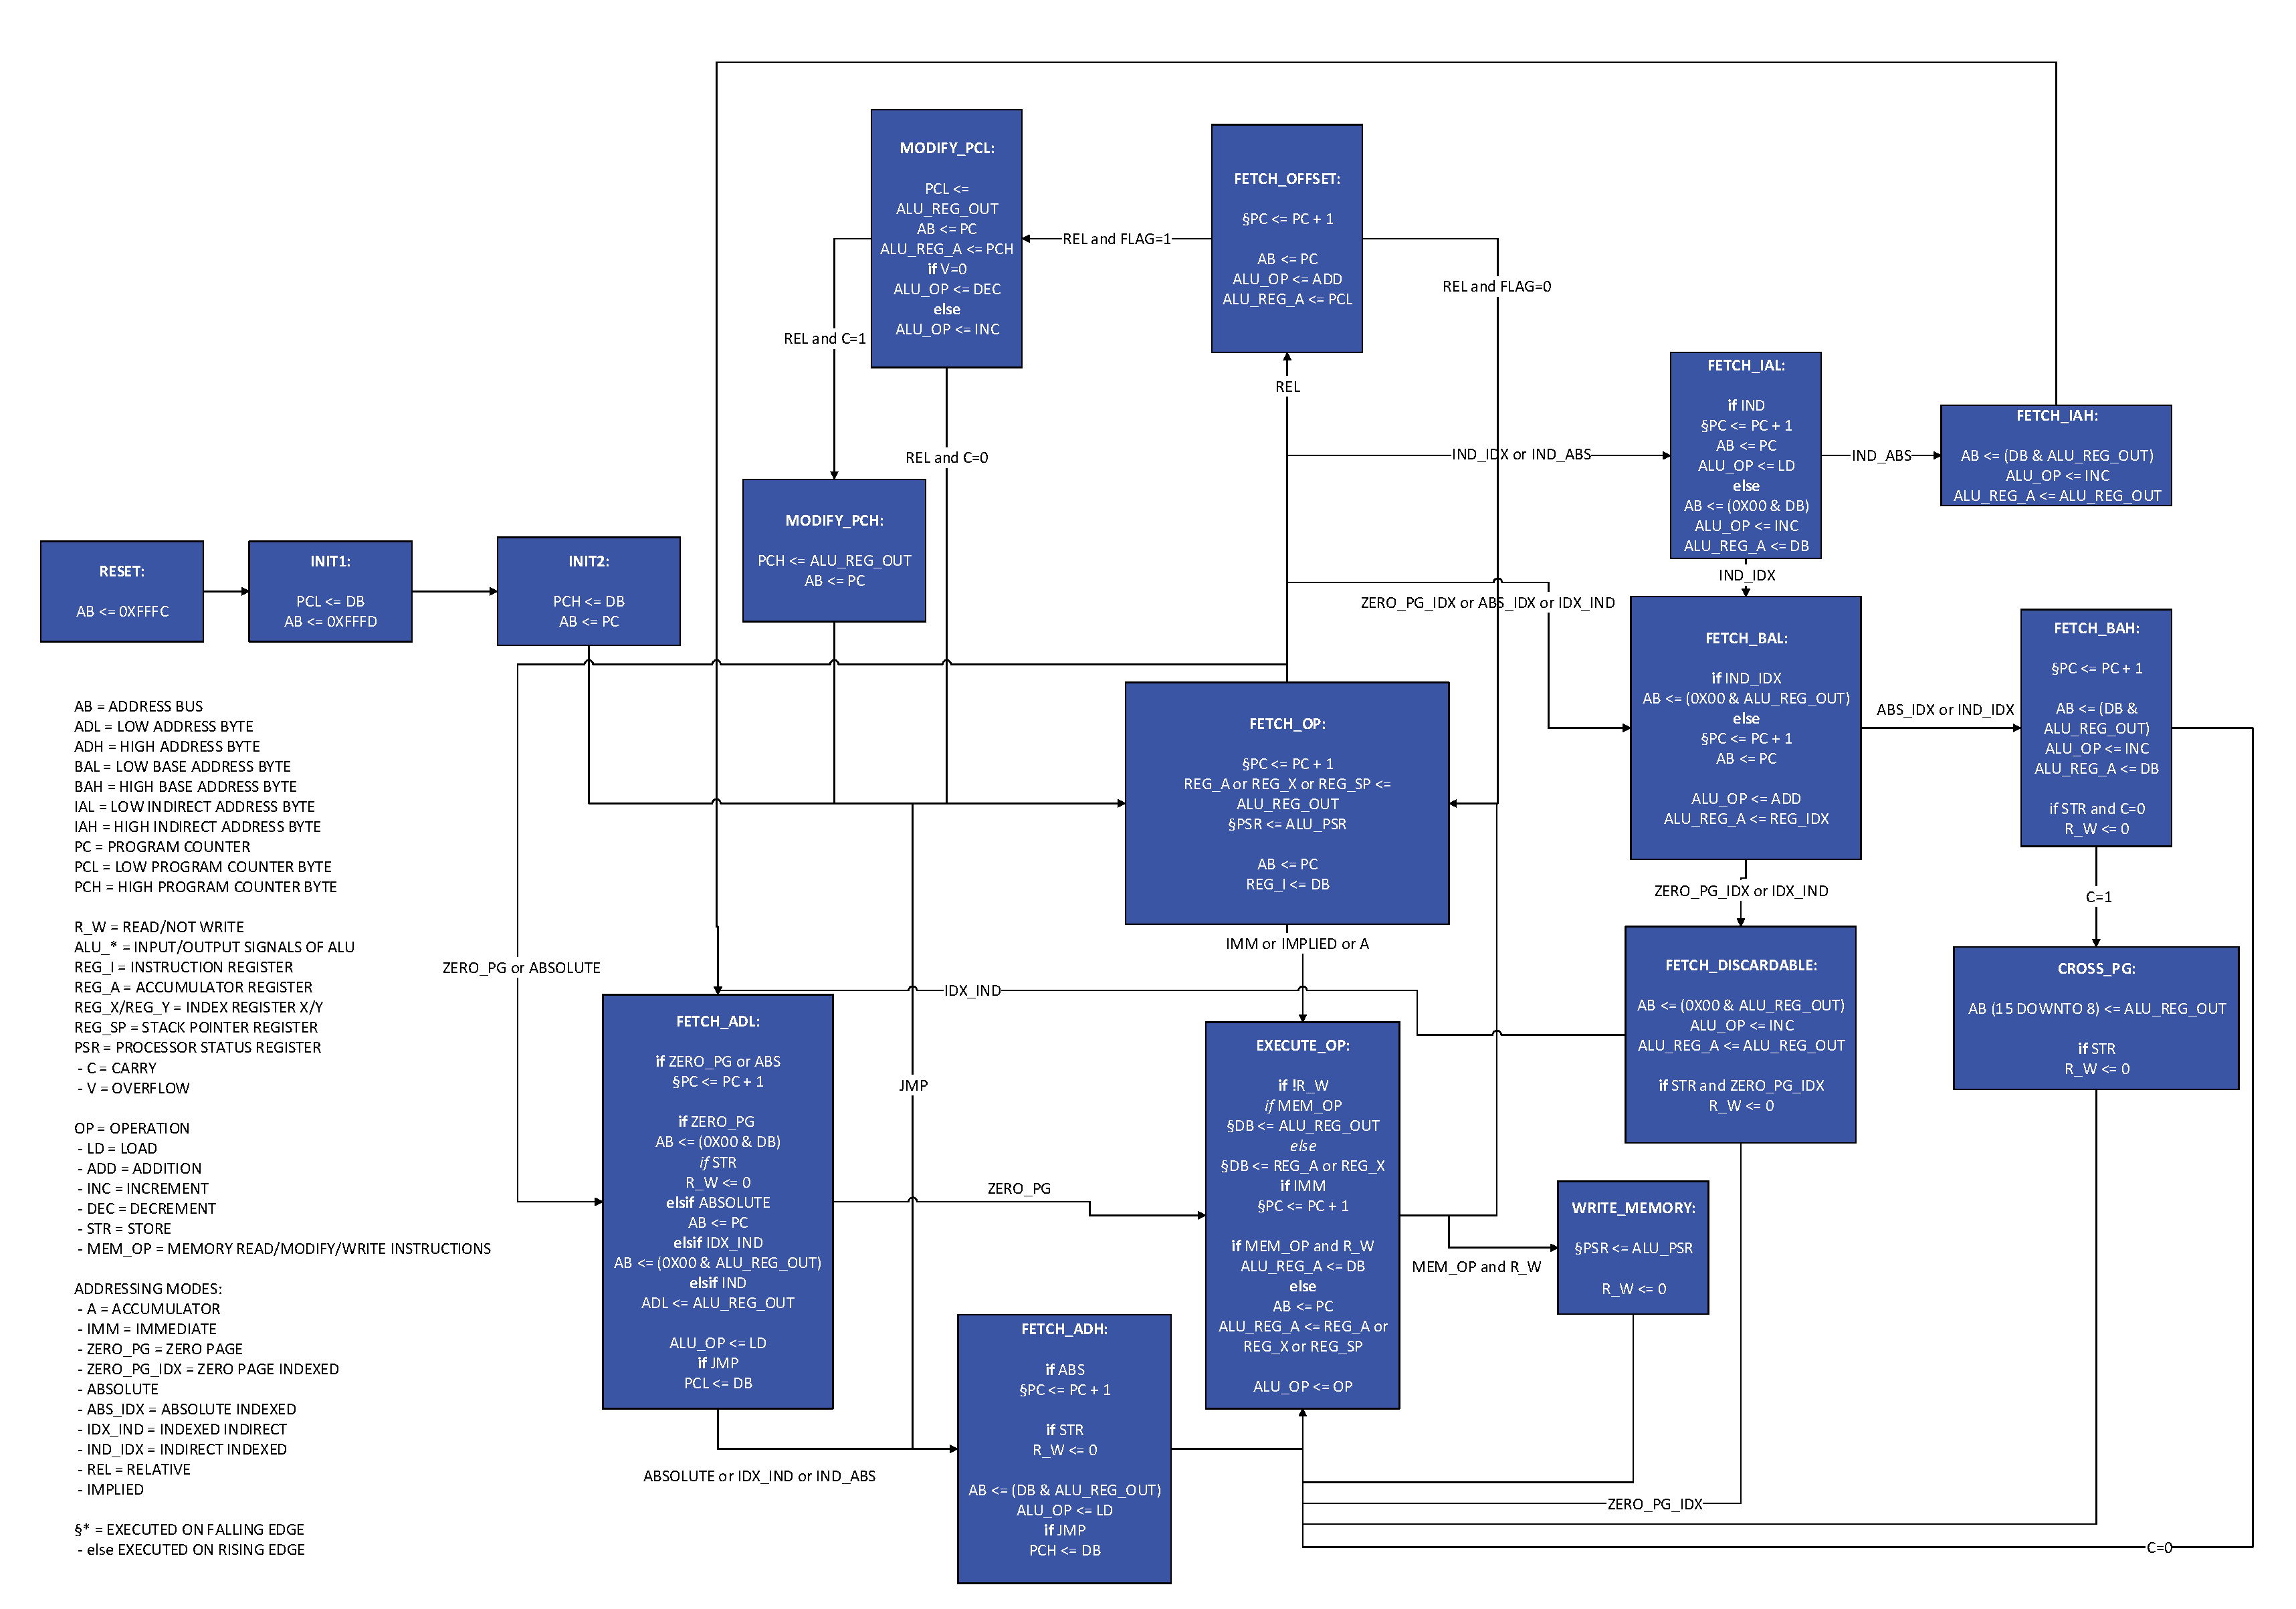
\includepdf[pages=-, angle=90]{../../_static/state_machine.pdf}
\end{landscape}
\newpage

\sphinxstepscope


\section{Audio Processing Unit}
\label{\detokenize{apu:audio-processing-unit}}\label{\detokenize{apu::doc}}
\sphinxstepscope


\chapter{Picture Processing Unit}
\label{\detokenize{ppu:picture-processing-unit}}\label{\detokenize{ppu::doc}}
\begin{sphinxthebibliography}{MOS Tech}
\bibitem[MOS Technology, Inc.75]{index:id13}
\sphinxAtStartPar
\sphinxstyleemphasis{MCS6501 \sphinxhyphen{} MCS6505 MICROPROCESSORS}. MOS Technology, Inc., 1975.
\bibitem[MOS Technology, Inc.76a]{index:id14}
\sphinxAtStartPar
\sphinxstyleemphasis{MCS6500 MICROCOMPUTER FAMILY HARDWARE MANUAL}. MOS Technology, Inc., 1976.
\bibitem[MOS Technology, Inc.76b]{index:id15}
\sphinxAtStartPar
\sphinxstyleemphasis{MCS6500 MICROCOMPUTER FAMILY SOFTWARE MANUAL}. MOS Technology, Inc., 1976.
\bibitem[Car84]{index:id11}
\sphinxAtStartPar
Joseph J. Carr. \sphinxstyleemphasis{6502 User\textquotesingle{}s Manual}. Reston Pub. Co., 1984.
\bibitem[Inc75]{index:id10}
\sphinxAtStartPar
Mos Technology Inc. Integrated circuit microprocessor with parallel binary adder having on\sphinxhyphen{}the\sphinxhyphen{}fly correction to provide decimal results. 1975. URL: \sphinxurl{https://patents.google.com/patent/US3991307}.
\bibitem[Kes99]{index:id7}
\sphinxAtStartPar
David Kessner. Free\sphinxhyphen{}6502. 1999. URL: \sphinxurl{https://www.sprow.co.uk/dump/index.htm\#Free6502}.
\bibitem[Mor12]{index:id9}
\sphinxAtStartPar
Nick Morgan. Easy 6502. 2012. URL: \sphinxurl{https://skilldrick.github.io/easy6502/}.
\bibitem[Qui11]{index:id8}
\sphinxAtStartPar
Quietust. Chip images. 2011. URL: \sphinxurl{https://www.qmtpro.com/~nes/chipimages/index.php}.
\bibitem[Tay04]{index:id5}
\sphinxAtStartPar
Brad Taylor. 2a03 technical reference. 2004. URL: \sphinxurl{https://www.nesdev.org/2A03\%20technical\%20reference.txt}.
\end{sphinxthebibliography}



\renewcommand{\indexname}{Index}
\printindex
\end{document}